%%%  Pacchetto di stile A4  %%%
\documentclass[12pt,a4paper,oneside]{book}
\usepackage[T1]{fontenc} 
\usepackage[utf8]{inputenc}
\usepackage{style/phdthesis} % Pacchetto di stile per le tesi

% Ridefiniamo la riga di testa delle pagine:
\usepackage{fancyhdr}
\pagestyle{fancy}
\usepackage{titlesec}
\usepackage{setspace}
\usepackage{wrapfig}
\usepackage{sectsty}
\usepackage{adjustbox}
\usepackage{lipsum}
\usepackage{multicol}
\usepackage[font=footnotesize]{caption}
\usepackage{listings} %Per inserire codice
\usepackage[usenames]{color} %Per permettere la colorazione dei caratteri 
\definecolor{dkgreen}{rgb}{0,0.6,0}
\definecolor{gray}{rgb}{0.5,0.5,0.5}
\definecolor{mauve}{rgb}{0.58,0,0.82}

\definecolor{lightgray}{rgb}{.9,.9,.9}
\definecolor{darkgray}{rgb}{.4,.4,.4}
\definecolor{purple}{rgb}{0.65, 0.12, 0.82}
\renewcommand\lstlistingname{}
\lstdefinelanguage{javascript}{
  keywords={typeof, new, true, false, catch, function, return, null, catch, switch, var, if, in, while, do, else, case, break, for},
  keywordstyle=\color{blue}\bfseries,
  ndkeywords={class, export, boolean, throw, implements, import, this},
  ndkeywordstyle=\color{darkgray}\bfseries,
  identifierstyle=\color{black},
  sensitive=false,
  comment=[l]{//},
  morecomment=[s]{/*}{*/},
  commentstyle=\color{purple}\ttfamily,
  stringstyle=\color{red}\ttfamily,
  morestring=[b]',
  morestring=[b]"
}

\lstset{frame=tb,
  captionpos=b,
  abovecaptionskip=0.5cm,
  aboveskip=0.8cm,
  belowskip=0.3cm,
  showstringspaces=false,
  columns=flexible,
  basicstyle={\small\ttfamily},
  numbers=left,
  numberstyle=\tiny\color{gray},
  keywordstyle=\color{blue},
  commentstyle=\color{dkgreen},
  stringstyle=\color{red},
  breaklines=true,
  breakatwhitespace=true
  tabsize=4,
  frame=lrbt,
  rulecolor=\color{gray}
}
\renewcommand{\chaptermark}[1]{\markboth{#1}{}}
\renewcommand{\sectionmark}[1]{\markright{\thesection\ #1}}
\fancyhf{}
\fancyhead[RO]{\thepage}
\fancyhead[LO]{\leftmark}
\renewcommand{\headrulewidth}{0.1pt}
\renewcommand{\footrulewidth}{0pt}
\headsep=20pt
\sectionfont{\Large} 
\subsectionfont{\itshape\large} 
\titleformat{\chapter}[display]
  {\normalfont\huge\bfseries}{\chaptertitlename\ \thechapter}{20pt}{\huge}
\titlespacing*{\chapter}{0pt}{-10pt}{40pt}

\setlength{\skip\footins}{1cm}
\setlength{\footnotesep}{0.4cm}

\graphicspath{{./figure/}}	% path directory figure
\linespread{1.5}	% interlinea
%%%%%%

\usepackage{graphics,graphicx}

\usepackage{amsmath,amsfonts,amssymb,amsthm} % pacchetti tipici per scrivere matematica  
\usepackage{latexsym}
\usepackage{array}
\usepackage{tocbibind}
\usepackage{listings}  % listati di codice

\usepackage{cite}
\usepackage{style/algorithmic}
\usepackage{style/algorithm2e}
\usepackage{color}

\usepackage{textcomp}
\usepackage{subfigure}
\usepackage{subfloat}

% TOC INFO: sono le info salvate nelle proprieta' del file pdf
\hypersetup{ 
  pdftitle=Master Thesis in Computer Science,
  pdfauthor=Saverio Meucci,
  pdfsubject=Forensic Analysis of Video File Containers
}    

%%%  Frontespizio  %%%

\university{}	% Universita' degli Studi di xxx (Firenze)
\faculty{Scuola di Ingegneria} %Nome della Scuola
\degree{}
\dept{} % nome dipartimento
\course{Corso di Laurea in Ingegneria Informatica} %Corso di Laurea

\accademicyear{Anno Accademico 2015/2016} %anno accademico
\supervisor{Prof. Alessandro Piva} % relatore
\supervisor{Prof. Fabrizio Argenti} %correlatore
\advisor{Ing. Marco Fontani} %correlatore
\advisor{Dott. Massimo Iuliani} %correlatore
\author{Saverio Meucci}

%titolo in italiano
%\title{\textbf{{\Huge Analisi Forense di Video File Containers}}}

%titolo in inglese
%\englishtitle{\textbf{{\Huge Forensic Analysis of Video File Containers}}}
\title{\textbf{{\Huge Forensic Analysis of Video File Containers}}}

\setcounter{tocdepth}{3}
\setcounter{secnumdepth}{3}

%%%  BEGIN DOCUMENT  %%%
\begin{document}

%%%  FRONT MATTER  %%%
\frontmatter
\maketitle  	% stampa la pagina di frontespizio

% DEDICA
\newpage{\thispagestyle{empty}\null\vfil
\begin{flushright}
\textit{{\large To myself.}}
\end{flushright}
}


\tableofcontents

%% Corpo della tesi

\mainmatter{
\chapter*{Abstract}
\addcontentsline{toc}{chapter}{Abstract}
\chaptermark{Abstract}

The investigation on digital contents is become more and more relevant with the increasing diffusion in our life of devices that can acquire images and videos. For this reason, there is the need to validate such digital contents so they can legitimately be used as evidence in a courtroom.
Research in the field of Multimedia Forensics have developed many techniques and methodologies that are able to verify the authenticity and the integrity of digital resources, such as images and videos, both analyzing the audio-video signal and the metadata information.
This thesis proposes an approach for forensic analysis of digital videos that uses information contained in file containers. In fact, video file format standards define only a limited set of mandatory features, leaving freedom of interpretation to the device manufacturers.
Information that comes from these difference in design decision is what our method exploits both with regard to Source Identification and Integrity Verification.

\chapter*{Sommario}
\addcontentsline{toc}{chapter}{Sommario}
\chaptermark{Sommario}

L'uso di contenuti digitali a fini investigativi sta diventando sempre più di attualità con l'aumentare della diffusione di dispositivi in grado di produrre immagini e video. Per tale motivo, è sempre più maggiore l'esigenza di validare tali contenuti digitali al fine di poter essere usati legittimamente come prove digitali.
La ricerca in ambito Multimedia Forensics si è adoperata nello studio di tecniche e metodologie che siano in grado di verificare l'autenticità e l'integrità delle risorse digitali, sia analizzandone il flusso dati che i metadati. 
Questa tesi propone una tecnica di analisi forense di video digitali che sfrutta i file container. Infatti, gli standard per i formati dei file video definiscono solo un numero limitato di features obbligatorie, lasciando così spazio per l'interpretazione da parte delle case produttrici di dispositivi. Queste differenze di interpretazione ed implementazione sono ciò che il nostro approccio sfrutta sia riguardo la Source Identification sia per l'Integrity Verification.
\chapter*{Introduction}
\addcontentsline{toc}{chapter}{Introduction}
\chaptermark{Introduction}

In an increasingly digital world, there are more and more applications where digital contents play a significant role.

Thanks to the spread of smartphones and digital cameras, the use of social networks that allow the sharing of digital images and videos is becoming more widespread. These resources, in general, contain information of personal nature; however, since these images and videos are more and more permeating our lives, their content may include information about an event that has occurred and therefore represents a significant source of evidence about a crime that can be used during an investigation.

In this context, many techniques for the analysis of multimedia content have been developed; these methods pose the goal of providing aid in making decisions about a crime so that a digital resource can be legitimately used as evidence in a courtroom.

Such is the task of the Forensic Analysis and in particular of Multimedia Forensics, i.e. to develop and apply techniques that allow, with a certain degree of precision, to determine whether the content of a digital resource is authentic or if it has been manipulated.

The questions that the Forensic Analyst must answer about digital contents are:
\begin{itemize}
\item authenticity assessment, or whether what they represent is true and correspond to reality.
\item integrity verification, i.e. if they have been altered in such a way that, however, does not compromise their authenticity.
\item the determination of the acquisition device, a problem that in Forensic Analysis takes the name of Source Classification or Source Identification.
\end{itemize}

To give a better understanding of these problems, we provide some application scenarios.

Regarding the Source Identification, imagine a situation in which the very act of creation of an image or video constitutes a crime, due to the content of the digital resource. In this scenario, it is crucial to establish the source device that generated the offending resource, so that this resource can be used as evidence. Depending on the context, determine the origin of a digital content could mean to find the particular acquisition device or the typology of the acquisition device or establish the last processing stage, such as a compression algorithm or an editing step.

In this context, it is also important the integrity assessment of a digital resource. In fact, the owner of the device that created the offending digital content could change the resource in such a way that it's not possible to trace back its source.

A more particular scenario, regarding the authenticity of a multimedia resource, is when the digital content is changed so as to deceive those who are watching it. The reasons for this manipulation can be different, such as the exaggeration or limitation of the severity of an accident or disaster, as well to change the context of the situation represented.

The tools available to the Multimedia Forensics are only those that can be extracted from the digital content itself. In fact, the fundamental idea of forensic analysis of digital content is based on the observation that both the acquisition process and the post-processing steps leave traces, called digital fingerprints. It is the task of the Forensic Analyst to analyze these fingerprints to determine the history and the authenticity of a digital content so that it can be used as evidence in a digital investigation.

In this regard, the analysis techniques of digital content mainly focused on two approaches. The first is the analysis of the data stream, i.e. the audio-visual signal, which is based on the research of artifacts and inconsistency in the digital content. The second is the analysis of the metadata, i.e. the determination of their compatibility, completeness, and consistency \cite{Piva} with regards to the context in which it is assumed the resource has been created.

Digital Image Forensics has extensively treated the presented issues; instead, regarding the Digital Video Forensics, the research for these problems is still under study and improvement. The motivation for this discrepancy lies in the much easier way that an image can be falsified than a digital video and the several video formats (MPEG, MPEG2, H26x, VP8, etc.) in contrast to the few main formats for digital images (mostly JPEG, PNG, TIFF).

This thesis proposes a technique for forensic analysis of digital video based on \emph{Gloe et al.} \cite{Gloe2014S68}, whose work focuses on the study of some video formats standard and the use of the internal structure of the video file container as a tool for the forensic analysis. This choice is justified by the fact that the video file container is very fragile so that it can contain a lot of information about the history of a digital video. Both the acquisition phase and the subsequent post-processing steps modify the content and the structure of the container. This fact can be exploited both regarding Source Identification and Integrity Verification.

The thesis is divided into chapters as follows. Chapter 1 provides an introduction to Multimedia Forensics, discussing both the state of the art techniques and the standards to be followed in all aspects of a digital investigation; it also explained in greater detail the work done by \emph{Gloe et al.} \cite{Gloe2014S68}, giving more information on video file containers. Chapter 2 will describe in detail the structure of the video file containers for MP4-like formats. In Chapter 3, it is presented the proposed approach along with all the choices made and the details of the implemented tool. Finally, Chapter 4 will show the dataset used and explain the motivation and the organization of the experiments along with a discussion of the results obtained.
\chapter{State of the Art}

\section{Introduction to Multimedia Forensics}

With the increasing spread of digital audio and video content, the analysis of these multimedia objects is rapidly assuming importance in the context of digital investigations, which consider both digital data and digital devices.

In digital investigations, multimedia content such as images, audio, and video are more and more being used as forensic evidence. It is, therefore, crucial to be able to extract information from such content in a reliable manner.

Multimedia Forensics has the aim to gain knowledge on a multimedia content life cycle exploiting the traces that the various processing steps leave on the data. In fact, the idea behind Multimedia Forensics is that each acquisition device and each processing operation on a digital resource leaves on the media content data some traces, often called fingerprints, which characterize its history.

Many algorithms and techniques have been developed by the scientific community based on the extraction of features from the stream of audio-visual data of the multimedia content. By taking advantage of these features, such techniques try to infer information about the source/acquisition device and about which encoding and editing processes the digital resource was subject to during its life cycle. Specifically for multimedia content such as images and videos, the main approaches set themselves the goal to identify the source of digital resource and to determine if the content is authentic or has been modified from its original without any a priori information about the content under analysis. This examination is possible using just these features and tools that allow checking for the presence or absence of such features or fingerprints that are intrinsically linked to the multimedia data by the acquisition device, the encoding step, and any post-processing or editing software tools. In fact, we can distinguish three types of traces left on a multimedia content: acquisition traces, encoding traces, and editing traces.

As explained, from a scientific point of view, research has produced a large number of techniques for the analysis of multimedia content. From the point of view of the application of such methods in the courtroom, however, there is still a significant gap. This gap is probably due to a lack of communication between the legal side and the scientific side, as well as a not full maturity of the techniques that are often based on results obtained in laboratory contexts a not in real-world scenarios.

Also, there is the need for greater sharing of standard in the field of digital multimedia forensics investigations that aid Multimedia Forensics to grow and reach maturity.

Several communities and groups have worked to put together guidelines and standard on important aspects of digital investigations, such as the chain of custody, data authentication, application of the scientific method, documentation, and reporting.
The ISO/IEC JTC1 Working Group 4 is one of those groups that seek to give international standards whose primary purpose is to promote the best procedures and methods for the investigation of digital evidence. It also encourages the adoption of approaches for the forensic analysis of multimedia content that are shared at an international level, in order to ease the comparison and the combination of results from different entities and organizations and also through various jurisdictions, so as to increase the reliability of such methods and the results.

Another group that aims at giving standards and guidelines for the digital investigations is the Scientific Working Group on Digital Evidence (SWGE) that deals with getting in contact different organizations that work in the field of Multimedia Forensics to promote communication and cooperation and to ensure higher quality and consistency within the forensic community.

The Scientific Working Group on Imaging Technologies (SWGIT), instead, focuses his work on image analysis technology and has the aim to facilitate the integration of such methods of analysis of images in the context of the judicial system. In fact, it provides best practices and guidelines for the acquisition, storage, processing, analysis, transmission, output image and archive of digital evidence.

Regarding the forensic analysis of images and videos, the process is defined to be composed of three main tasks: technical preparation, examination, interpretation. The technical preparation is concerned with all those operations necessary to prepare videos and images to the other tasks. The examination is the main part of the forensic analysis and deals with the application of techniques that aim to extract information from images/videos. The interpretation concerns the analysis of digital content from experts in order to provide conclusions on the features extracted from the images/videos under examination.

In this context, it becomes essential the figure of the Forensic Analyst, i.e. one who can develop and apply these methods for the analysis of digital content, interpret the results and make a summary of the results from different techniques to increase the reliability of the conclusions. It is also able to perform all of the analysis tasks following the standards shared by the forensic community. The Forensic Analyst can find the traces left on the multimedia data and acquire information on the object under examination such as which is the source/acquisition device, whether the content is authentic and if the resource is intact, and so on.

\subsection{Applications}

The major applications for forensic analysis are source identification, authentication assessment, and integrity verification of multimedia resources.

The source identification process has as objective the retrieval of information about the device of origin that generated the multimedia content under examination. It is possible to identify the source at various levels of detail. For example, sometimes it is possible to distinguish between types of sources or to make a distinction between different models of the same kind of source or between the various devices that belongs to the same type and model.

The authentication problem has to do with the task of determining whether the multimedia content is an accurate representation of an original event. The analysis process is typically based on finding inconsistencies in the features extracted from the audio-visual signal.

The integrity problem concerns the task of determining whether a multimedia content has been changed or not from the moment that the acquisition device has created it. The analysis is based on the search for traces left by the editing tool or post-processing step during the life cycle that are not compatible with the source device that, for this application, is assumed to be.

\subsection{Tools}

Multimedia files can be viewed as a package composed of two main parts: the header, which contains the metadata, i.e. the information about the contents of the file; the content itself, i.e. the data stream which forms the audio-visual signal.
In general, the feature extraction is based on the analysis of traces left on both the actual data and the metadata of the multimedia file.

As for the inspection of the data stream, specifically for images and videos, the examination consists of two most important aspects:
\begin{itemize}
\item interpretation of the content, which is the analysis of the content to understand what the data represents, who are the subjects and the objects involved, what is the environment. In general, the goal it to retrieve all the information that can be extrapolated from human observation.
\item identification of sensitive details from the scene represented, such as audio-visual anomalies, the direction of the light, shadows, perspective inconsistencies, smudge marks, and so on.
\end{itemize}

Also in the context of the inspection of the audio-visual signal, a useful technique is to enhance the content, such as the improvement of the signal to detect relevant details or objects, the extraction of dimensional relationships between subjects and objects, the visual comparison between known objects and objects represented in the scene.

The other tool regards the extraction and analysis of the metadata. Metadata can be easily extracted and can contain a lot of information regarding the data stream such as source device, color space, resolution, compression parameters, date, GPS coordinates, frame rate, format tags, bitrate, sample rate, the number of channels. Obviously, the type and the number of metadata depends on the type of the file under examination and which processes have undergone during its life cycle. Once the metadata is obtained, it is the Forensic Analyst work to verify the compatibility, the completeness, and the consistency \cite{Piva} of this information with regards to the context in which it is known or assumed the resource come from. In fact, metadata might be different if a digital resource originates from a social network rather than directly from the acquisition device.

\section{Forensic Analysis of Video File Container}

\subsection{Video File Containers}

The forensic analysis has focused mainly its attention on the analysis of images, developing techniques that used either the data stream, the metadata, or both. Regarding the latter, JPEG \cite{jpeg} and EXIF \cite{exif} metadata have become very used. Since each acquisition device and processing software use their customized quantization tables, given an image, it is possible to exploit these differences to limit the search of the origin \cite{farid}. Also, by considering the number of EXIF entries and the compression parameters, \emph{Kee et al.} \cite{kee2001} associate images whose origin is not known to a certain class of source device.
The forensic analysis of digital videos is currently more and more relevant. Early works have followed procedures similar to the ones used for the images, exploiting artifact and inconsistency in the data stream and examining the information extrapolated from the metadata.
However, regarding the use of metadata especially for the identification of digital sources, there are concerns over falsifiability. In fact, it is just a matter of finding the right software tools, often publicly available, to easily edit high-level information such as Exif metadata.
However, the known processing software and metadata editors, both for images and videos, do not have a functionality to modify low-level information, such as the internal order of the core file structures. These characteristics are thus extremely valuable and offer a higher reliability than standard metadata information.

The work of \emph{Gloe et al.} \cite{Gloe2014S68} expands this idea to the video forensics by exploiting the low-level characteristics represented by metadata and file format information such as video file container. By identifying specific manufacturer and model characteristics, as well as traces left by processing or editing software, it is possible to assess the authenticity or the integrity of a video and to identify its origin, in terms of a particular device or a type of devices.

Indeed, \emph{Gloe et al.} noticed that the video format standards for the data container formats prescribe only a limited number of features, thus leaving a lot of freedom to the manufacturer. The Forensic Analyst can exploit this fact as a resource, given a video, to identify the source and to assess its authenticity or its integrity. 

As well as for the JPEG and EXIF low-level characteristic, the known tools do not allow to change the video file containers since they are a core file structure. For this reason, these low-level features reduce the concerns about the falsifiability of such information as only for a subject in possess of advanced programming skills will be able to modify the internal structure and content of video file containers. Even in this scenario, it would still be very complex to preserve consistency amongst all of the metadata information, thus making the operation of falsifiability not trivial even for a highly technical figure.

\emph{Gloe et al.} \cite{Gloe2014S68} explore in details both the AVI \cite{avi} and the MP4-like file formats. Digital cameras mainly use the AVI video stream. This thesis focused its work on the analysis of videos generated by mobile phones; thus, we will give a brief overview of only the MP4-like file containers structure and the ways its characteristics can be exploited for digital forensic purposes. An explanation in great details about the structure and content of file containers of MP4-like formats will be given in Chapter 2.

Apple introduced the MOV \cite{mov} container format in 1991. Using this format as a basis, the MP4 \cite{mp4} and 3GP formats have also been created. This group of file formats will be referred to as MP4-like file formats.

The video file containers of this formats are composed of atoms (sometimes called boxes) that are identified by a unique 4 bytes characters, preceded by the size of the atom. These atoms can have fields and can be nested, i.e. an atom may contain another atom. Thus, four types of atoms can be encountered:
\begin{itemize}
\item atoms without fields and that do not contain other atoms.
\item atoms without fields but that contain other atoms.
\item atoms with fields that do not contain other atoms.
\item atoms with fields that also contain other atoms.
\end{itemize}

The most typical structure of the MP4-like containers is as follows:
\begin{itemize}
\item \emph{ftyp} atom: it is semi-mandatory, i.e. the latest ISO standards expect it to be present and to be explicit as soon as possible in the file container. It refers to the specific file types with which the video file, to which the container belongs, is compatible.
\item \emph{mdat} atom: it contains the data stream and specifies its size.
\item \emph{moov} atom: it is the atom with the most complex structure of the container. It is a nested atom which contains many other atoms. In this atom, and in its sub-structure, is included the metadata needed for the decoding of the data stream contained in the \emph{mdat} atom.
\end{itemize}

This structure is not always respected. The file container of the MP4-like formats are very complex and have many elements and differences that depend on the source and the manufacturing company; thus it can constitute a valuable tool for the Forensic Analysis.
The differences of containers across multiple types of video files can be found in many ways, as explained as follows:
\begin{itemize}
\item the relative position of the atoms: although the standard gives specifications about the location of specifics atoms (especially the main ones described above), these indications are not always respected. Above all, there is a change in position for those atoms whose position is not specified but the standard. This fact is true both for the atoms at the first level, such as \emph{ftyp}, \emph{mdat}, \emph{moov}, and for the atoms of the sub-structure contained in the \emph{moov} atom.
\item the presence of additional non-standard atoms at all level of the container.
\item the differences in the fields values of the atoms.
\end{itemize}

All these possible differences and types of differences give rise to a large set of combinations that the Forensic Analyst can use to analyze a digital video resource.

\subsection{Applications for Video File Container Analysis}

The problem of the authentication is based on the analysis of the audio-visual signal to determine if the data is an actual representation of an original event. Thus, it is not in our domain because video file containers are treated as metadata. With metadata, you can not assess anything about the events represented in a video.

The integrity problem, instead, can be dealt with. As described above, the container of a video file is the container created by the last tool during the file lifecycle. If a video was also slightly modified by a software, it will have its own container. This container may contain additional atoms or change the positions and the fields values of the other atoms compared to the file container of the video before it was processed. Therefore, if the file container content and structure of an acquisition device is known, it is possible to compare the container of the query video file with the container of a reference video file (i.e. a video generated by the known or assumed acquisition device). In this way it is possible to verify the integrity of the query video file, i.e. whether the file, during the time between its generation from the source device and the present, has been modified or not.

The problem of the source classification makes sense because, since the standards define only a few mandatory features for the file container, the manufacturing companies are left with a lot of freedom. This space for interpretation means that every class of device will have its own different container structure and values. This fact can be used to construct a set of features to distinguish between devices. For examples, in the case of video created by smartphones, it can be used to determine the belonging of a video to a brand, or to a specific brand and model, or to a specific brand, model, and operating system.
It becomes necessary to find a way to represent the various classes in a training set properly. Besides, a compatibility measure must be defined to compute the likelihood of a query container to belong to a particular class of devices.

The proposed approach in this thesis will do just that, giving all the theory and the necessary information of how to implement a pipeline to solve the integrity and the source identification problem of a video file using its file container.
\chapter{Video File Formats}


The ISO Base Media File Format is a container for multimedia formats which can contain both audio and video data. It is a general format that represents a basis for a number of other file formats.
As described in the standard ISO/IEC 14496 Part 12 \cite{iso}, it is designed to contain media information for a video in a flexible and extensible format so that the interchange, management, editing, and presentation of a media are facilitated. The information represented includes timing, structure, and media information for a presentation, i.e. one or more motion sequences that can also be combined with audio.

The ISO Base Media File Format has a object-oriented type structure. In fact, files conform to this standard are formed as a sequence of objects, called boxes or sometimes atoms, that contain all the data about the media. Some of these boxes can also contain other boxes. A box consists of a header, followed by the box data. The header contains a unique type identifier, representing the type of the box, and the size of the box. Some boxes may also contain information fields about version number and flags. For these fields, the semantic is the following:

\begin{itemize}
\item \emph{size}: an integer that specifies the number of bytes used by a box, including the fields and all contained boxes.
\item \emph{type}: a four printable characters that identifies the box type.
\item \emph{version}: an integer that specifies the version of the format of the box.
\item \emph{flags}: a set of flags.
\end{itemize}

The sequences of boxes in a file must contain one representation metadata wrapper, i.e. the Movie Box (\emph{moov}). The other boxes that can be found at the first level are File Type Box (\emph{ftyp}), Free Space Boxes (\emph{free}), Movie Fragments (\emph{moof}), Meta-data (\emph{meta}), or Media Data Boxes (\emph{mdat}).

The MP4 File Format, described in the standard ISO/IEC 14496-14 Part 14 \cite{mp4}, and MOV File Format, described in the QuickTime File Format specification \cite{mov}, are derived from the ISO Base Media File Format. In fact, the general structure of the ISO file is fully implemented by both file formats. Each file format introduces new boxes and redefines the values of some fields that are already present in the ISO standard.

In the following, we will give additional information about the structure and the content of the boxes contained in an ISO file.

\section{Box Definitions}

An overall view of an example of a object-oriented structured file of this format can be view in Table \ref{boxtable}. For the complete encapsulation structure, \cite{iso} can be consulted.

\begin{table}[]
\centering
\begin{tabular}{|l|l|l|l|l|l|l|l|l}
\hline
  ftyp &      &      &      &      &      & * & file type and compatibility\\ \hline
  moov &      &      &      &      &      & * & container for all the metadata \\ \hline
       & mvhd &      &      &      &      & * & movie header \\ \hline
       & trak &      &      &      &      & * & container for an individual trak \\ \hline
       &      & tkhd &      &      &      & * & track header\\ \hline
       &      & mdia &      &      &      & * & container for the media information \\ \hline
       &      &      & mdhd &      &      & * & media header \\ \hline
       &      &      & hdlr &      &      & * & handler \\ \hline
       &      &      & minf &      &      & * & media information container \\ \hline
       &      &      &      & vmhd &      &   & video media header \\ \hline
       &      &      &      & smhd &      &   & sound media header \\ \hline
       &      &      &      & hmhd &      &   & hint media header \\ \hline
       &      &      &      & dinf &      & * & data information box \\ \hline
       &      &      &      &      & dref & * & data reference box \\ \hline
       &      &      &      & stbl &      & * & sample table box \\ \hline
       &      &      &      &      & stsd & * & sample descriptions \\ \hline
       &      &      &      &      & stts & * & time-to-sample \\ \hline
       &      &      &      &      & stcs & * & sample-to-chunck \\ \hline
       &      &      &      &      & stcz &   & sample sizes (framing) \\ \hline
       &      &      &      &      & stco & * & chuck offset \\ \hline
       &      &      &      &      & co64 &   & 64-bit chunk offset \\ \hline
       &      &      &      &      & stss &   & sync sample table \\ \hline
       &      &      &      &      & sdtp &   & independent and disposable samples \\ \hline
       &      & udta &      &      &      &   & user-data \\ \hline
       & udta &      &      &      &      &   & user-data \\ \hline
  moof &      &      &      &      &      &   & movie fragment \\ \hline
  mdat &      &      &      &      &      &   & media data container \\ \hline
  free &      &      &      &      &      &   & free space \\ \hline
  meta &      &      &      &      &      &   & metadata \\ \hline
\end{tabular}
\caption{Box types and structure. The boxes with an asterisk (*) are mandatory.}\label{boxtable}
\end{table}

The table shows the boxes that shall occur at the top-level of the file in the left-most column, with indentations representing containments. The boxes that are marked with an asterisk (*) are mandatory. In the following, each box of the table will be described, also giving examples taken from the file container of a video from a Samsung Galaxy S3 that uses the MP4 file format.

\subsection{First Level}

At the first level we will find:

\subsubsection*{File Type Box (ftyp)}

Since a media file structured accordingly to this file format standard can be compatible with more than one specification, it is not possible to speak of a single type or brand for a file.
The File Type Box (\emph{ftyp}) is a mandatory and unique box that identifies which type represents the best use for a file, along with other compatible specifications. Each brand is described by a four characters code.

The box \emph{ftyp} should be positioned at the top-level of a file before every other box of variable lenghts, such as Movie Box, Free Box, or Media Data Box. Only a box with a fixed-size, such as file signature, may placed before it. The box \emph{ftyp} has three fields:

\begin{itemize}
\item \emph{major\_brand}: identifies the best use specification.
\item \emph{minor\_version}: identifies the version of the major specification.
\item \emph{compatible\_brands}: a list of other compatible specifications.
\end{itemize}

\subsubsection*{Movie Box (moov)}

The Movie Box (\emph{moov}) is a mandatory and unique box that contains the necessary metadata for a presentation and is placed at the top-level of a file. Although it is not explicitly required, it is normally located close to the beginning or end of a file. It is also a container for other boxes.

\subsubsection*{Movie Fragment Box (moof)}

The Movie Fragment Box (\emph{moof}) is an optional box that extends the media in time, providing additional information that would previously have been present in the Movie Box. It is placed at the top-level of a file and contains a Movie Fragment Header Box (\emph{mfhd}) and one or more Track Fragment Boxes (\emph{traf}). The Movie Fragment Boxes must be placed in the file accordingly to their sequence number.

\subsubsection*{Media Data Box (mdat)}

The Media Data Box (\emph{mdat}) contains the media data. Since a presentation can contain zero or more Media Data boxes, it is a optional box. It has a field that specifies the size of the contained media data.

\subsubsection*{Free Space Box (free)}

The Free Space Box (\emph{free}) is an optional box that can be placed at the top-level of a file or can be contained in other boxes. Usually, the content of this box can be ignored and therefore deleted, without affecting the presentation.

\subsubsection*{Meta Box (meta)}

The Meta Box (\emph{meta}) is an optional box that contains annotative metadata. This box may be located at the top-level of the file, or inside the Movie Box (\emph{moov}) or the Track Box (\emph{trak}). If present, it is required to contain a Handler Reference Box (\emph{hdlr}) that indicates the format of the content of the Meta Box.

\subsection{Second Level}

At the second level, we will find:

\subsubsection*{Movie Header Box (mvhd)}

The Movie Header Box (\emph{mvhd}) is a mandatory and unique box that is located inside the Movie Box. It is used to specify characteristics of an entire video. The fields contained in the box \emph{mvhd} are the following:

\begin{itemize}
\item \emph{version}: an integer that specifies the number of bytes for this Movie Header Box.
\item \emph{creation\_time}: an integer that represents the creation time of a video.
\item \emph{modification\_time}: an integer that represents the most recent time the video was modified.
\item \emph{timescale}: an integer that specifies the time-scale for the entire media. It indicates how many units pass in one second.
\item \emph{duration}: an integer representing the length, in terms of time, of the video.
\item \emph{rate}: it indicates the preferred rate to play the video.
\item \emph{volume}: it indicates the preferred audio volume to play the video.
\item \emph{matrix}: it represents a geometrical transformation matrix for the video.
\item \emph{next\_track\_ID}: a non-zero integer that specifies an ID value to use for the next track to be added to the video.
\end{itemize}

It is advised that the Movie Header Box should be placed first in its container.

\subsubsection*{Track Box (trak)}

The Trak Box (\emph{trak}) is a mandatory box for a file that is located inside the Movie Box. A video contained one or more tracks, such as audio or video tracks, with each track independent from the others. Tracks can either be media tracks, containing media data, or hint tracks, containing information for streaming protocol. Every presentation must have at least one media track within an ISO file.

\subsubsection*{User Data Box (udta)}

The User Data Box (\emph{udta}) is an optional box that can either be contained inside a Movie Box or a Track Box. It contains objects that specify user information about the presentation or the track. It contains a set of boxes with more box types that indicate more precisely their content.

It is advised that the User Data Box should be placed last in its container.

\subsection{Third Level}

At the third level, we will find:

\subsubsection*{Track Header Box (tkhd)}

The Track Header Box (\emph{tkhd}) is a mandatory and unique box that specifies the characteristics of a track. It is contained inside the Track Box. It contains the following fields:

\begin{itemize}
\item \emph{version}: an integer that specifies the version of the box. Can either be 0 or 1.
\item \emph{flags}: an 24-bit integer whose values indicates a track that is enabled (\emph{Track\_enabled}), a track that must be used for in the video (\emph{Track\_in\_movie}), or a track that must be used in the preview of the video.
\item \emph{creation\_time}: an integer that indicates the creation time of a video.
\item \emph{modification\_time}: an integer that represents the most recent time the video was modified.
\item \emph{track\_ID}: an integer number that uniquely identifies a track.
\item \emph{duration}: an integer that indicates the length, in terms of time, of the video.
\item \emph{layer}: it specifies the order \emph{front-to-back} of the video tracks.
\item \emph{alternate\_group}: an integer that specifies a group of tracks. It can either be 0, meaning that no relations between tracks are present, or 1, meaning that there are relations between tracks of different groups.
\item \emph{volume}: it specifies the relative audio volume of the track.
\item \emph{matrix}: it represents a transformation matrix for the video.
\item \emph{width} and \emph{height}: they specify the resolution of the video track.
\end{itemize}

It is advised that the Header Header Box should be placed first in its container.


\subsubsection*{Media Box (mdia)}

The Media Box (\emph{mdia}) is mandatory and unique box within the file and it is contained inside the Track Box. It contains all the objects that specify information about the media data in a track.

\subsection{Forth Level}

At the forth level, we will find:

\subsubsection*{Media Header Box (mdhd}

The Media Header Box (\emph{mdhd}) is a mandatory and unique box contained inside a Media Box. It declares all the information relevant to the media in a track. The box \emph{mdhd} contains the following fields:

\begin{itemize}
\item \emph{version}: an integer that indicates the version of this box.
\item \emph{creation\_time}: an integer that indicates the creation time of the media track.
\item \emph{modification\_time}: an integer that indicates the most recent time the media track was modified.
\item \emph{timescale}: an integer that specifies the time-scale for the entire media. It indicates how many units pass in one second.
\item \emph{duration}: an integer representing the length, in terms of time, of the media track.
\item \emph{language}: it specifies the language code for the media track.
\end{itemize}

It is advised that the Media Header Box should be placed first in its container.

\subsubsection*{Handler Reference Box (hdlr)}

The Handler Reference Box (\emph{hdlr}) is a mandatory and unique box that is contained inside a Media Box or a Meta Box. When inside a Media Box, it specifies the nature of the media track. For example, a video track will be handled by a video handler and a sound track will be handled by a sound handler. When inside a Meta Box, it indicates the format of content of the Meta box.

It contains the following fields:

\begin{itemize}
\item \emph{version}: an integer that specifies the version of the box.
\item \emph{handler\_type}: when inside a Media Box, it is an integer containing 'vide' for video tracks, 'soun' for sound track or 'hint' for hint track; when inside a Meta Box,  it contains a value indicating the format of the content of the Meta Box.
\item \emph{name}: a string of characters that associates a human-readable name for the media track type.
\end{itemize} 

\subsubsection*{Media Information Box (minf)}

The Media Information Box (\emph{minf}) is a mandatory and unique box that is located inside the Media Box. It contains characteristic information about the media track.

\subsection{Fifth Level}

At the fifth level, we will find:

\subsubsection*{Video Media Header Box (vmhd)}

The Video Media Header Box (\emph{vmhd}) is media information header box located inside the Media Information Box. It contains general information about the video track. The box \emph{vmhd} has the following fields:

\begin{itemize}
\item \emph{version}: an integer that specifies the version of the box.
\item \emph{graphicmode}: it specifies a composition mode for the video track.
\item \emph{opcolor}: is an RGB value that is available for use by the graphics modes.
\end{itemize}

\subsubsection*{Sound Media Header Box (smhd)}

The Sound Media Header Box (\emph{smhd}) is a media information header box located inside the Media Information Box. It contains general information about the audio track. The box \emph{smhd} has the following fields:

\begin{itemize}
\item \emph{version}: an integer that specifies the version of the box.
\item \emph{balance}: a number that places mono audio tracks in a stereo space.
\end{itemize}

\subsubsection*{Hint Media Header Box (hmhd)}

The Hint Media Header Box (\emph{hmhd}) is a media information header box located inside the Media Information Box. It contains general information about the hint track.

\subsubsection*{Data Information Box (dinf)}

The Data Information Box (\emph{dinf}) is a unique box that is mandatory within a Media Information Box. It can also be located inside a Meta Box and contains the location of the media information in a track.

\subsubsection*{Sample Table Box (stbl)}

The Sample Table Box (\emph{stbl}) is a mandatory and unique box situated inside the Media Information Box. It contains entries tables that specify the location of the sample, the type of the sample, determine their size and offset within the container. Such tables are contained in sub-boxes that indicate information about sample description (\emph{stsd}), sample size (\emph{stcz}), sample to chunk (\emph{stcs}), chunck offset (\emph{stco}), etc.

\subsection{Sixth Level}

At the sixth level, we will find:

\subsubsection*{Data Reference Box (dref)}

The Data Reference Box (\emph{dref}) is a mandatory and unique box located within a Data Information Box. It contains a table of data references (URLs) that specifies the location of the media data used within the video file.
\chapter{Proposed Approach}

\section{Overview}

Our method specifically focused on Source Identification and Integrity Verification. In the following, we will explain the theory behind our proposed approach, that is the main idea of why and how to use video file containers for Multimedia Forensics.

As mentioned in the previous chapters, video file containers contains structured information about the content such as content-related metadata (acquisition time, modification time, place, etc.), number of tracks and signals (audio and video), and codec data (quantization tables, etc.) that is necessary to decode and present the signal. Since the file format standards leave room for freedom to the manufacturers about how the file container is composed, we can harness both its content and, mostly, its structure. The idea behind the use of file containers is that both the source device or the platform from which a video originates leave traces on its containers, so that we can determine its history.

For Source Identification, we are in this scenario: given a query video we want to assess if it belong to a class $C$ based on its file container, where for a class we mean a source of origin. Specifically, during this thesis, we have focused our study on video file generated from smartphones. In this case, we can imagine the possible classes as having a hierarchic structure; so a class could be seen a specific brand, a specific model of a certain brand, or a specific operating system on a certain brand of some brand of smartphones.

Basically, given a query video and a class $C$, we pose a binary question: does this query video belongs to the class $C$? In order to answer that question, we split the ground truth set of videos in two classes $X_{C}$ and $X_{\overline{C}}$, i.e. of videos belonging to class $C$ and not respectively.

To determine which of the two classes the query video belongs, we need a compatibility score. We create $\Omega$ that is the set of all the attributes $\omega$ of the atoms contained in each file containers of the ground truth media. We determine the discrimination power of each attributes $\omega$ for the class $C$,

$$  W_{C}(\omega) = \dfrac{\sum\limits_{i=1}^{N_{C}}\mid X_{i} \cap \omega \mid}{N_{C}} $$

with $X_{i} \in X_{C}$ and $N_{C}$ the number of videos of the ground truth that belongs to the class $C$.

Similarly, we compute the discrimination power of each attributes $\omega$ for the classe $\overline{C}$,

$$  W_{\overline{C}}(\omega) = \dfrac{\sum\limits_{i=1}^{N_{\overline{C}}}\mid X_{i} \cap \omega \mid}{N_{\overline{C}}} $$

with $X_{i} \in X_{\overline{C}}$ and $N_{\overline{C}}$ the number of videos of the ground truth that belongs to the class $\overline{C}$.

With the discrimination power, we can determine how significant an attribute is for a certain class.

The procedure described above is what we refer to as the training phase. For the test phase, given a query video $X = \left\lbrace \omega_{1},...,\omega_{n} \right\lbrace $, we solve the two hypothesis test problem:

$$  H_{0}:X \in \overline{C} $$
$$  H_{1}:X \in C $$

The we determine the likelihood of observing $\omega_{j} \in X, j = 1,...,t$ for each of the two classes.

$$ P(\omega_{j}\vert H_{0}) = \Omega_{\overline{C}}(\omega_{j}) $$
$$ P(\omega_{j}\vert H_{1}) = \Omega_{C}(\omega_{j}) $$ 

Supposing, that $\omega_{j}$ are independently distributed we can compute a likelihood

$$ L(X) = \dfrac{\prod\limits_{\omega_{j}} \Omega_{C}(\omega_{j} }{\Omega_{\overline{C}}(\omega_{j}} $$

to determine whether a query video $X$ to belong to the class $C$.

For Integrity Verification, the approach is simpler because we don't need to deal with classes. In this scenario, we have a query video $X$ that supposedly come from a certain device and we want to assess if this supposition is true or if the video has undergone some other processing step during its lifecycle. In order to do that, we create a reference video $Y$ with the device that supposedly is the source of the video $X$; to assess the integrity, we need to determine the compatibility of the file containers of the query video $X$ with the file container of the reference video $Y$. 

For each attributes of $Y$, we check their presence in the file containers of $X$; then we do the same operation in reverse, that is checking the presence of the attributes of $X$ in the file containers of $Y$. The results will be a percentage representing a measure of compatibility between query and reference, i.e. by how much the two file containers under examination differs. It will be up to the Forensic Analysis, by also checking for which attributes the two file containers differ, to determine if this compatibility score is enough to assess the integrity of the query video or not.

In order to put into place the described approaches, we developed several applications that can be used both as a Java library and a command-line tool. Finally, we implemented a web application so that a user can utilize these methods more easily.

\section{Video Format Tool}

\subsection{Features}

The Video Format Tool is a software application that we have implemented mainly to extract the file container from an input video. However, this program also presents various other features which serve to manipulate file containers; these features are both implemented as low-level functions, so that they can be used as functions from a Java library, and as high-level functions, that are used as interfaces for the command-line tool.

The implemented features are:
\begin{itemize}
\item[-] \emph{Parse}: given input MP4-like format video file (MP4 and MOV), it extracts the file container using the \emph{MP4Parser} library \cite{mp4parser} and it saves it in an XML file, using the \emph{JDOM} library \cite{jdom}.
\item[-] \emph{Batch parse}: given as input a folder containing video files, it parses all the videos in the folder and sub-folder, saving them into XML files by recreating the same folder structure.
\item[-] \emph{Draw}: it is used to draw in a window a tree, given an XML file as input that represents a video file container.
\item[-] \emph{Merge}: given two XML input files, it combines them into a single XML file. By taking one as the base for the merge, it adds to it the atoms that only the other XML file has; also, for atoms that are in common, it considers the attributes and, by looking at their values, it adds them to the base XML files, so that for each attributes we will have a vector of values.
\item[-] \emph{Update}: it is an advanced method to use the merge. Instead of giving two XML files as input, it takes a folder that contains XML files and merges them into a single XML as explained above. It also considers sub-folders.
\item[-] \emph{Compare}: given two XML files, it compares them and it returns a measure of how much they differ.
\end{itemize}

\subsection{Implementation} 
 
During the development of the application, we have made several implementation choices. In the following, it will be described the reason behind them, in addition to further details. The features that will be explained are only the main ones: parse, merge and appear:

\subsubsection{Parse}

The \emph{parse} feature make use of the \emph{Mp4Parser} library, a Java API to read, write and create MP4-like files.

To explain how the \emph{parse} feature is implemented, we will follow the process of extraction of a file container from the input of a video to the creation of the corresponding XML file.

First, the function \emph{parse()} is called; this function servers as an interface for the command-line application to extract a file container from a MP4-like video and parse it into an XML file. It takes two String as parameters: the first representing the path of the file video that we want to parse, and the second representing the path of the directory where to save the resulting XML files. After validating the input file path, using the \emph{MP4Parser} library, it extracts the ISO file from the input video. Then it called the \emph{parser()} function, passing the extracted ISO file.

The \emph{parser()} function is used to parse an ISO file into a \emph{JDOM Element}. Firstly, it creates a root \emph{JDOM Element} and then it calls the constructor for the \emph{BoxParser} class, passing the ISO file. Finally, it calls the \emph{getBoxes()} method of the \emph{BoxParser} object.

The \emph{getBoxes()} method is a recursive function that takes as parameters: an \emph{AbstractContainerBox} object, from the \emph{MP4Parser} library, that represents an abstract base class that is suitable for boxes (i.e. atoms) of the file container that act as container for other boxes; the root \emph{JDOM Element} created by the \emph{parser()} function.
The first time that this method is called, the first parameter will be a \emph{Null} object. It will extract a list of children boxes from the ISO file. The boxes extracted from the ISO file will be the boxes at the first level of nesting of the file containers, generally ftyp, mdat and moov boxes.
For each child box, it creates a new \emph{JDOM Element} using as a name the identifier of the box, i.e. the 4-byte code. Then, it extracts and parse the attributes of the box and will set them as fields of the \emph{JDOM Element}. At this point, there is the recursive step: if the box under examination is also a container of other boxes, the \emph{getBoxes()} method will be called again this time passing the box as an \emph{AbstractContainerBox} instead of null, and the newly created \emph{JDOM Element}, that will act as a root for the lower levels of the file containers; if the box does not contain other boxes then the newly created \emph{JDOM Element} is added to the root and a new child box will be parsed.
At the end of the recursion, the first \emph{JDOM Element} that we passed from the \emph{parser()} function, will contain all the information about the file container, preserving its tree-like structures and its attributes values.

Finally, the flow of execution will return to the \emph{parse()} function which will ensure that the \emph{JDOM Element} will be saved in an XML file in the passed output folder.

During the development of this application, several implementations choices were made that we will explain in the following.

The parsing of the attributes for each box takes place using some wrapper functions. In fact, the \emph{MP4Parser} library implements a \emph{toString()} method for each specific \emph{Box} class; however this method is not always consistent and it will not be even present for some box types. To overcome this issue, we realize a \emph{Wrapper} interface that require the implementation of said \emph{toString()} method. For each of the Box types that we encounter, we created the corresponding wrapper classes that implement the Wrapper interface, as well as a default \emph{Wrapper} class that deals with unrecognized boxes. This way, we have full control over the \emph{toString()} method and how the attributes of a box are retrieve. One way that we customized the extraction of the attributes, it is the addition of an attributes to each box; we add an attribute called count in order to determine the presence or the absence of the boxes, that will be useful afterwards, especially for boxes that do not have attributes.
Also, it extensible in the sense that, if we are in the presence of a new box that we previously never encounter, we can easily implement its wrapper class and its \emph{toString()} method.

One of the aspects that make file containers a valuable resource for the forensic analysis is the presence of low-level characteristics such as its structure and the locations of each atom in the containers. To take advantage of this feature, the name of each \emph{JDOM Element} object will be formed by the 4-byte code of the corresponding atom along with a index number that represents the relative position with respect to the other children. This is especially useful for exploit the differences in the container structure: if two file container have a different order for, as an example, the \emph{ftyp}, \emph{mdat} and \emph{moov} atoms, then, by using this indexing, we will be able to notice and harness the variation in the container structure.

Instead, the position of the attributes of each atom is not relevant. Whether it is used the toString() functions of the Mp4Parser library or the one that we implemented as classes that extend a Wrapper interface, the order of the attributes is still arbitrarily decided by either one of the two proxies. This fact means that the order has nothing to do with choices that the manufacturer made and it cannot help to determine the source device or platform of a video file.

\subsubsection{Tree interface}

In order to represent the XML files as objects, from each \emph{JDOM Element} can be built a custom \emph{Tree} object, so that they can be manipulated more easily accordingly to our needs.

The \emph{Tree} interface is implemented in order to maintain the same nested structure of a XML file that represents a file containers. It is used as the \emph{Component} class in the \emph{Composite} pattern to implements trees. Such as a file container or a XML file, a tree can have children, which are other sub-tree, and fields, which are couples of name and value.

Each tag of an XML file can be a \emph{Node} or a \emph{Leaf}, both classes that implements the \emph{Tree} interface. Each \emph{Tree} object has a name for identification, a String variable whose value is taken from the name of the tag, a father, that is another Tree object or a \emph{Null} object for the root Tree object, a list of children \emph{Tree} objects and a list of \emph{Field} objects, that correspond to the attributes of XML tag.

The \emph{Tree} interface also requires many feature to add, remove, retrieve and modify each \emph{Tree} object along with its children and its list of \emph{Field} objects.

\subsubsection{Merge}

The \emph{merge} feature combines two XML files, representing two file containers, and merges them into a single XML file. It is the features that will be used, during the training phase, to create $\Omega$, the set of all the attributes $\omega$ of the atoms contained in each file container of the ground truth videos.

The \emph{merge()} function serves as an interface for the command-line program to merge two XML files into a single one. It takes as parameters two \emph{String} representing the path of the first XML file and the path of the second XML files, respectively.

Firstly, it creates two Tree objects from the input XML files; then it proceeds to call the \emph{mergeTree()} function, by passing to it the two \emph{Tree} objects. The first \emph{Tree} object is taken as the base to which the elements of the second \emph{Tree} object will be added. The function begins by extracting the children of the second \emph{Tree} object; for each child, it checks its presence in the first \emph{Tree} object.
If it is not present it will add that child \emph{Tree} object to the first \emph{Tree} object at the corresponding level and by setting the right father.
If it is present, it will check the fields of the corresponding child in the first and second \emph{Tree} object. For each field couple, it will compare their values and, if they differ, it will add it to the values of that particular field for the first Tree object. This way the first Tree object will have fields values that represent vector of values.

The function now proceeds recursively; the \emph{mergeTree()} function will be called again by passing the corresponding child in each of the \emph{Tree} objects. The recursion will stop once it will have reach the \emph{Leaf} object for each of the tree branches.

The final results will be contained in the first \emph{Tree} object passed, that now represents the union of the two XML files, both in terms of atoms and of attributes values.

Then, the merge() function will save the resulting merged \emph{Tree} object into an XML file.

Since the result is of \emph{mergeTree()} in another \emph{Tree} object, this features can be used repeatedly to merge many XML files by adding to the same merged one. This merged XML files represents the $\Omega$ set.

\subsubsection{Compare}

The \emph{compare} feature serves to compare two XML files and give a measure of how much the file containers they represent differ. It is the feature used to verify the integrity of query video by confronting it to a reference video for which the source device is known.

Similar as for the other features, the \emph{compare()} function serves as an interface for the command-line program. It takes as parameters two \emph{String} representing the path of the first XML file and the path of the second XML files, respectively.

The first input XML file represents the video that will be taken as a reference and the second input will represent the query video. Both XML files are converted into two Tree objects and are passed to the \emph{compareTree()} function. The \emph{compareTree()} is a recursive function that behaves similarly to the previously mentioned recursive functions: it iterates through the reference Tree object children and checks for difference for each of the corresponding child in the query video. If there is not a corresponding child, then all the attributes of the child of the reference Tree object will be counted as difference. If there is a corresponding child, it will be counted a difference every time that a pair of attributes from the reference Tree object and the query Tree object differs in their values. Also, attributes for which a difference is found are saved in a list, along with the corresponding values from both of the Tree object.

Besides the number of differences, it is also counted the total number of attributes of the reference Tree object. The final results will be a percentage, computed dividing the number of differences found with the total number of attributes, that represents how much the two file containers differ.

The results are then returned as JSON formatted output.

\subsection{Command Line Examples}

In the following section, we will explain how to use the command-line interface for the Video Format Tool by giving some examples of usage.

\begin{itemize}

\item[-] Extract a file container from a video and save it into an XML file.
\begin{lstlisting}
vft --parse -i input.mp4 -o /output_folder
\end{lstlisting}

\item[-] Batch parse a directory of videos. It also recreates the same sub-folders structure.
\begin{lstlisting}
vft --batch -i /input_folder -o /output_folder
\end{lstlisting}

\item[-] Draw a tree from an input XML file.
\begin{lstlisting}
vft --draw -i input.xml
\end{lstlisting}

\item[-] Merge two XML files, with or without consider the attributes.
\begin{lstlisting}
vft --merge -wa -i input.xml -i2 input2.xml -o /output_folder
\end{lstlisting}

\item[-] Merge all XML files in a given directory into a single XML file saved in the output folder, with or without attributes. It also considers XML files in sub-directories.
\begin{lstlisting}
vft --update-config -wa -i /input_folder -o /output_folder
\end{lstlisting}

\item[-] Compare two XML files and return a measure of how much they differ.
\begin{lstlisting}
vft --compare -i input.xml -i2 input2.xml
\end{lstlisting}

\item[-] Print the help message.
\begin{lstlisting}
vft --help
\end{lstlisting}

\end{itemize}


\section{File Origin Analysis Tool}

\subsection{Functional Requirements}

The File Origin Analysis Tool is the software application implements the theory behind our proposed method regarding Source Identification based on video file containers and it is developed to be used as a command-line program.

The main features are:
\begin{itemize}

\item[-] Training: given two sets of videos, one representing a class $C$ and the other a class $\overline{C}$, it will creates $\Omega$, saved as a XML files. Then, for each attribute $\omega$ it will compute the discriminant power regarding the class $C$ and the class $\overline{C}$, respectively.

\item[-] Test: given a query video $X$, for each attribute $\omega_{j} \in X$ it will check the corresponding discriminant power estimated by the previous training phase for both the class $C$ and the class $\overline{C}$. By combining all the discriminant powers of all the attributes $\omega_{j}$, it will compute a measure, representing the likelihood that $X$ belongs to the class $C$.

\end{itemize}

\subsection{Implementation}

\subsubsection{Training}

The task of the training phase it is to compute the discriminant power of each attribute $\omega \in \Omega$. The work-flow of the feature is as follow. The \emph{Train} class is the one that deals with the training phase. Its constructor will take as arguments two \emph{VideoClass} objects, one for the class $C$ and the other for the class $\overline{C}$, that will contains a list of XML files for each ground truth video of the class, and a \emph{String} for the output folder in which the XML file that represents $\Omega$ will be saved.
Using the \emph{train()} method of the \emph{Train} class, it will first iteratively use the merge feature of the \emph{Video Format Tool} library to compute $\Omega$ and represent it as a XML file, that will be referred to as the configuration file. The resulting XML file will contain all of the atoms found in the file container of the ground truth videos. For each attribute, as explained in the Video Format Tool section, its value will be a list of possible values found for the attribute of that particular atom in every file containers of the ground truth. Also, to each attribute will be associated two vectors of weights, the same size as the number of possible values, initialized to zero. These vectors will be used to compute the discriminant power of each attribute value regarding both class $C$ and class $\overline{C}$.

This computation is done by the \emph{computeWeights()} method of the \emph{Train} class, first for the class $C$ and then for the class $\overline{C}$. It takes two \emph{Tree} object of the \emph{Video Format Tool library}, one representing the configuration XML file and the other a video of class $C$. For each atom of the configuration \emph{Tree} object, it will search for the corresponding atom in the class $C$ \emph{Tree} object. Then, for each attribute of the class $C$ \emph{Tree} object it will check for its value in the list of possible value for that attribute contained in the configuration \emph{Tree} object and will increment the weight that correspond to that value. Each weight $w_{i}$ is normalized by the number of videos of the class under examination, so that $w_{i} \in \left[0, 1\right] $.

Finally, the configuration Tree object will contain the discriminant powers of every attributes values for each atom for the ground truth with regard to the class $C$. The same process will be applied to the videos of the class $\overline{C}$ and then both configuration Tree object will be saved in two separate XML files, one for class $C$ and one for class $\overline{C}$, terminating the training phase.


\subsubsection{Test}

In the test phase, given a query video $X$, we want to determine, based on its file container, if $X$ belongs to the class $C$ or not. In order to do so, we need a likelihood measure that takes into account all the discriminant powers of the attributes value of the file container of the video $X$ with regards to class $C$ and class $\overline{C}$.

The constructor of the class \emph{Test} takes as arguments the path of the XML file, that represent the file container of the query video, and the paths for the configuration XML files for both class $C$ and class $\overline{C}$.
The method \emph{test()} will build all passed XML files to \emph{Tree} objects. Then, it will create a \emph{StandarLikelihood} object, a class that implements the \emph{Likelihood} interface. In this way, we can change and customized how we want the likelihood to be computed.

The implemented \emph{StandardLikelihood} works as follow. Using the \emph{computeLikelihood()} method, it explores all the atoms of the query Tree object. For each of these atom, it will search for the corresponding one in both configuration Tree objects. For each attribute of the atom under examination, it will compute the ratios between the weights from both classes associated with that value, with the weight for the class $C$ as a numerator and the weight for the class $\overline{C}$. All the ratios for each attribute of the query file container will then be multiplied between them, obtaining a likelihood measure $L(X)$, which is then smoothed with the natural logarithm. 
The final result $l(X) = ln(L(X))$ can be used to determine whether X belongs to the class $C$.


\subsubsection{Implementation Details}

The list of possible values associated to an attribute of the configuration files is computed by merging the values for that certain attribute found both in the videos of the class $C$ and the class $\overline{C}$. It is possible that a given value for an attribute is only present in the videos of a class but never in the other. This fact means that the weight, i.e. the discriminant power, associated to that attribute value will be zero for the latter.
Also, the origin of the query video could be unknown, meaning that its source will differ from all the video of the ground truth. The file container of the query video could have both atoms and attributes values that are not present in the configuration files. When computing the ratio for these new attributes, it follows that they will not have a weight associated.

To deal with these issue, we have identified four different scenarios that can happen when computing the ratios between the values weights.

The default case is the easiest one and it occurs when both the weight associated to class $C$ and the weight associated to class $\overline{C}$ are greater that zero.

When the weight associated to the attribute value for the class $\overline{C}$ equals to zero, then the ratio between the weights will have the form of $ \dfrac{w_{i}}{0} $, with $w_{i}$ the weight associated to the attribute value for the class $C$. A division by zero is not acceptable. To overcome this issue, we modified the computation to $$ \dfrac{w_{i}}{\dfrac{1}{N_{C} + 1}} $$, where $N_{C}$ is the number of videos in the class $C$. In this way, the denominator will have the smallest possible value and the ratio will still pull the likelihood towards the class $C$.

Instead, when the weight associated to the attribute value for the class $C$ equals to zero, the ratio will have the form of $ \dfrac{0}{w_{j}} $, with $w_{j}$ the weight associated to the attribute value for the class $\overline{C}$. In this case, since the numerator is zero, the ratio will equal to zero too. This is an unwanted scenario because, since all the ratios are multiplied between them, a single ratio that equals to zero is enough to make the general likelihood zero too. We decided to solve this problem by modifying the computation of the ratio for this case to $$ \dfrac{\dfrac{1}{N_{\overline{C}} + 1}}{w_{j}} $$, where $N_{\overline{C}}$ is the number of videos in the class $\overline{C}$.

Finally, when an atom or an attribute value is not present in the configuration files, we have the case where both weights equal to zero. Since we want to determine if a given query video $X$ belongs to the class $C$, any information on the file container that is not present in the configuration files for the class $C$ will be treated as if it means that the video does not belong to the class $C$, even if the same information is also not present in the configuration file for the class $\overline{C}$.

When multiplying the ratios for a certain atom, the resulting value can be seen as a likelihood of observing that specific atom with its attributes values in either of the two classes. However, the values of the attributes for an atom are not, in general, independently distributed. This means that the values of some attribute can change in groups. If we simply multiplied all the ratios, it will be as if we are counting the same information multiple time, pushing the likelihood towards the class $C$ or the class $\overline{C}$ improperly.

To solve the issue, we multiply the likelihood ratios of each atom by also taking into consideration the decorrelation factor.
Given a vector of likelihood ratios $(x_{1},\ldots,x_{n})$ we compute the likelihood $$ L(\overline{x}) = \prod\limits_{i=1}^{n} x_{i}^{\alpha_{i}} $$ with $$ \alpha_{i} = \dfrac{(n-1)\gamma_{i}+1}{n} $$ $$ \gamma_{i} = - \dfrac{n}{log n} P(x_{i})log P(x_{i}) $$ and where $P(x_{i})$ represent the probability of finding that value of ratio in the vector.
We have three cases:

\begin{itemize}

\item[1)] $P(x_{i}) = \dfrac{1}{n} $ with $x_{i} \neq x_{j}$, $ \forall i \neq j $.
Then we will have $$ \gamma_{i} = - \dfrac{n}{log n} \dfrac{1}{n} log\dfrac{1}{n} $$ resulting in $\alpha_{i} = 1$.
The likelihood will be computed as $$L(\overline{x}) = \prod\limits_{i=1}^{n} x_{i} $$

\item[2)] $P(x_{i}) = 1 $ with $x_{i} = x_{j}$, $ \forall i,j $.
Then we will have $ \gamma_{i} = 0 $ and $\alpha_{i} = \dfrac{1}{n} $.
The likelihood will be computed as $$L(\overline{x}) = \prod\limits_{i=1}^{n} x_{i}^{\dfrac{1}{n}} = x_{1}^{\sum \dfrac{1}{n}} = x_{1} $$

\item[3)]  $x_{i} = x_{j}$, $ i,j = 1,\ldots,k $ with $P(x_{i}) = \dfrac{k}{n} $ for $i = 1,\ldots,k$ and $P(x_{j}) = \dfrac{1}{n}$ for $j > k$.
Then we will have $$ \gamma_{i} = -n \dfrac{n}{log n} \dfrac{k}{n} log \dfrac{k}{n} = k (log \dfrac{k}{n})log n $$ and 
$$ \alpha_{i} = \dfrac{(n-1)(k log \dfrac{k}{n})log n + 1}{n} $$
The likelihood will be computed as $$L(\overline{x}) = x_{i}^{\sum \dfrac{1}{n}} = x_{1}^{\left[ (n-1)(k log \dfrac{k}{n})log n + 1 \right] \dfrac{k}{n}} \cdot \prod\limits_{j=k+1}^{n} x_{j}  $$

\end{itemize}

\subsection{Command Line Examples}


In the following section, we will explain how to use the command-line interface for the File Origin Analysis Tool by giving some examples of usage.

\begin{itemize}

\item[-] Compute the configuration files for given classes $C$ and $\overline{C}$.
\begin{lstlisting}
foa --train --listA classC.json --listB classNotC.json -o /output_folder
\end{lstlisting}

\item[-] Given two classes $C$ and $\overline{C}$, test if a video $X$ belongs to class $C$.
\begin{lstlisting}
foa --test -i input.xml --configA configC.xml --configB configNotC.xml
\end{lstlisting}

\item[-] Print the help message.
\begin{lstlisting}
vft --help
\end{lstlisting}

\end{itemize}

\section{Web Application}

To facilitate the application of the proposed approach for forensic analysis using the tool previously explained, we have also implemented a web application. Its task is to act as a graphical user interface and allow a user to customize the query and present the results in a more readable format. The web application was developed using the \emph{Javascript} runtime \emph{Node.js} \cite{node} and with the framework \emph{Express.js} \cite{express} for the server's back-end. It uses a \emph{SQLite} database to store information about the ground truth videos and the classes of devices that are available.

The web application implements functionalities for the Source Identification and the Integrity Verification using the feature of the \emph{Video Format Tool} and of the \emph{File Origin Analysis Tool}, which are called \emph{Classify} and \emph{Compare} respectively.
It also has a test functionality that helps to speed up the experiments that will be explained in a later section of this thesis.

\subsection{Features}

It is possible to select the feature that we want to use from the navigation bar at the top of the page. In the following, it will be described how each feature work.

\begin{itemize}

\item[-] \emph{Classify}: this feature is use for Source Classification purposes. As shown in \ref{fig:classify}, the user can upload the query video or directly the XML file representing the file container from the Upload box and, from the Class box, select the class for which they want to determine the belonging of the query video. The results will then be outputted in the Output box. 

\begin{figure}
  \centering
  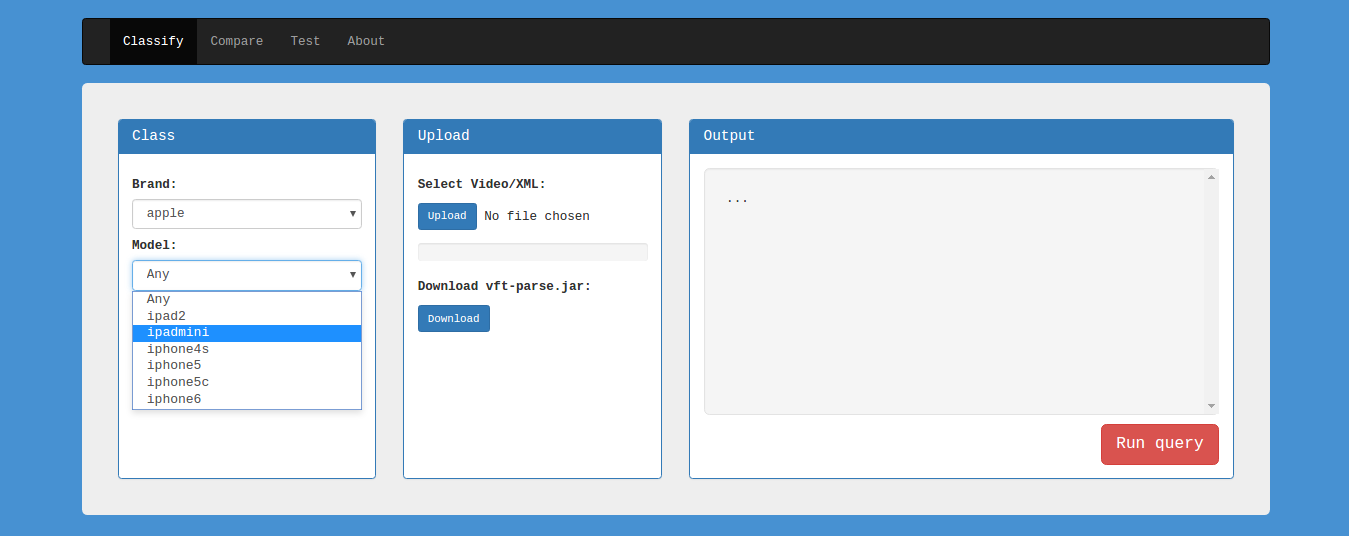
\includegraphics[width=1\textwidth]{classify}
  \caption{The user can select the class to test for the \emph{Classify} feature.}\label{fig:classify}
\end{figure}

It can work in two different ways: if the user specifically select a class (a brand, a brand and a model, or a brand a model and an operating system), the method will execute in manual mode; if the user leaves the default values \emph{Any} from each selection, the method will execute in automatic mode.

The manual mode is generally used when the user already have an assumption about the query video source device and wants to assess its correctness. Choosing a specific class is equal to asking a binary question: does the query video belongs to this selected class? The application will proceeds to split the ground truth accordingly and will compute and return the likelihood for the query video regarding the selected device class.

The automatic mode is typically used when no assumption is made about the query video origin. Instead one binary problem, we pose as many binary problem as there are classes of devices in our ground truth dataset of videos. For each class, the likelihood will be computed and then sorted with regards to all other. The outputted result, as shown in \ref{fig:classify-output}, will be a list of classes sorted by likelihood in decreasing order.

\begin{figure}
  \centering
  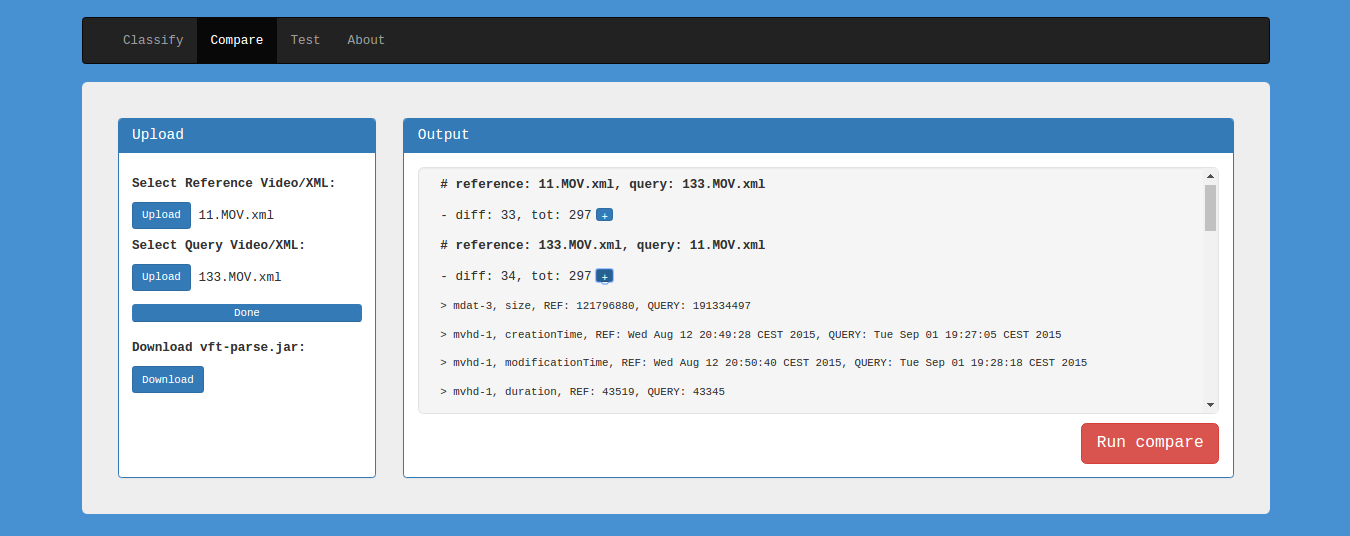
\includegraphics[width=1\textwidth]{classify-output}
  \caption{For the automatic mode of \emph{Classify}, the results will be shown as a list of classes sorted in decreasing order of likelihood}\label{fig:classify-output}
\end{figure}

The \emph{Classify} feature also allow the user to upload and compute the likelihood for more than one query video at a time.

Particular attention must be reserved in how the ground truth is split once a class $C$ to test is chosen. In fact, we have found that the results can be greatly affected by the reference population, in our case the complementary class $\overline{C}$. This problem affects also other application of forensic analysis, mainly in Speaker Recognition. Thus, it is important to decide if the reference population must represents a sample of the entire population or a sample of the population that presents similar characteristics to the population of the class under examination. For our case, this question translates to choosing if the class $\overline{C}$ should contain a sample of all the videos in the ground truth that do not belong to the class $C$, or a sample of all videos in the ground truth that do not belong to the class $C$ but that are similar to the videos in class $C$.

We decide for the latter approach.
If a class is compose of brand, model, and operating system the complementary class $\overline{C}$ is chosen by taking the videos of the ground truth that have the same brand and model but different operating system.
If a class is compose of brand and model, leaving the default value Any to the operating system field, the complementary class $\overline{C}$ is chosen by taking the videos of the ground truth from the same brand but that have a different model.
Finally, if for a class is specified only the brand field, the complementary class $\overline{C}$ is composed by a sample of all the videos from the ground truth that are from a different brand. This is, of course, the most general case and equivalent to choosing a sample of the entire population as the reference.

\item[-] \emph{Compare}: this functionality allows the user to verify the integrity of a query video, exploiting the \emph{compare} feature of the \emph{Video Format Tool} application. The user must upload two videos, one representing the reference and the other the query for which the integrity must be assess. Once the operation is concluded, in the Output box will be shown the results about the comparison by displaying the number of difference that the query videos have with regards to the reference video and vice-versa; it also possible to show the atoms and the attributes for which the differences are found, as shown in \ref{fig:compare}.

\begin{figure}
  \centering
  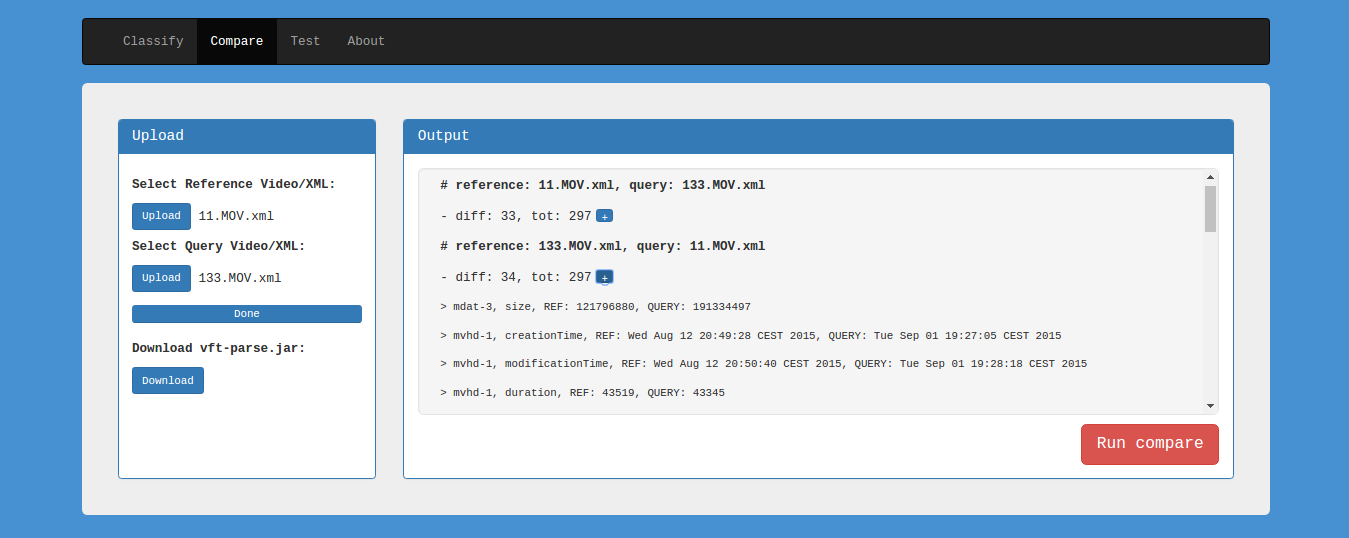
\includegraphics[width=1\textwidth]{compare}
  \caption{For the \emph{Compare}, it is also shown the atoms and the attributes for which the differences are found.}\label{fig:compare}
\end{figure}

\item[-] \emph{Test}: the \emph{Test} functionality is just an utility to iterate the \emph{Classify} over a number of videos without the need to manually upload each video. In fact, the query videos are store in a table of the web application database along with information about their true class. The output results will be the same as for the \emph{Classify} but with the addition of statistics about the accuracy of the classification.

\end{itemize}

For both the \emph{Classify} and \emph{Compare} functionality, it is possible to upload a query video directly as a video file. However, since this is a web application, there could be limitation in the upload speed of an user making the process of using this tool slow. As mention previously it possible to upload the XML file representing a video file container as query but, in general, a user might not possess the instrument to acquire such XML file. For this reason, we have also develop a small Java \emph{Swing} GUI application that can be downloaded from the web application. This app allows the user to parse a video file into a XML file representing its file container, using the parse feature from the \emph{Video Format Tool}, as well as parsing an entire folder. In this way, due to the small size of a generic XML file, it is possible to execute a query seamlessly.
\chapter{Experiments and results}

\section{Dataset}

The dataset used in this thesis is composed of video coming from smartphones and tablets with operating system \emph{Android} and \emph{iOS}. 
Videos that have an \emph{Android} acquisition device have a file container that follows the standard of the MP4 \cite{mp4} file format while videos that have an \emph{iOS} acquisition device have a file container that follows the standard of the MOV file format \cite{mov}.
The full list of devices of our dataset can be seen from Table \ref{devices}). 

\begin{table}[]
\centering
\begin{tabular}{|l|l|l|l|}
\hline
\textbf{OS}       & \textbf{BRAND}    & \textbf{MODEL}             & \textbf{\#}			 \\ \hline
Android &         &                   & 150         \\ \hline
        & Samsung &                   & 132         \\ \hline
        &         & Galaxy S3         & 18          \\ \hline
        &         & Galaxy S3 mini    & 36          \\ \hline
        &         & Galaxy S4 mini    & 18          \\ \hline
        &         & Galaxy Tab 3      & 36          \\ \hline
        &         & Galaxy Tab A      & 9           \\ \hline
        &         & Galaxy Trend Plus & 15          \\ \hline
        & Huawei  &                   & 18          \\ \hline
        &         & G6                & 18          \\ \hline
iOS     &         &                   & 110         \\ \hline
        & Apple   &                   & 110         \\ \hline
        &         & iPad 2            & 15          \\ \hline
        &         & iPad mini         & 15          \\ \hline
        &         & iPhone 4S         & 14          \\ \hline
        &         & iPhone 5C         & 18          \\ \hline
        &         & iPhone 5          & 31          \\ \hline
        &         & iPhone 6          & 17          \\ \hline
        &         &                   & 260         \\ \hline

\end{tabular}
\caption{The list of devices in the dataset divided by operating system, brand and model.}
\label{devices}
\end{table}


For each device, we have videos that are directly acquired and the same videos that have been modified by different means:

\begin{itemize}
\item videos that have been uploaded and then downloaded from 	\emph{Youtube}.
\item videos that have been modified using the software tool \emph{Ffmpeg} \cite{ffmpeg}.
\item videos that have been modified using the software tool \emph{Exiftool} \cite{exiftool}.
\end{itemize}

\section{Integrity Verification based on File Container}

In order to determine how our approach performs with regard to Integrity Verification we have set up some experiments. A copy of the videos in our dataset have been modified through different means, thus losing their integrity. In this experiments we check whether the information of the file containers are sufficient to tell the original videos and the modified ones apart.

The tools that we have used to modify the videos are \emph{Ffmpeg} and \emph{Exiftool}. The modification we have made are as minimal as the tools allow.

In general the experiments have been performed as follow. Given a list of videos $(x_{1},\ldots,x_{n}) \in C_{i}$, with $C_{i}$ a certain device, we have generated a corresponding list of minimally processed videos $(\overline{x_{1}},\ldots,\overline{x_{n}})$ using a certain tool. For each couple of videos $(x_{i}, x_{j})$ of the same device we have computed the differences using the \emph{compare} feature of the Video Format Tool. These measures tell us how much the videos of the same device differs. Then we compute the difference for each couple of $(x_{i}, \overline{x_{j}})$ and for each couple $(\overline{x_{i}}, x_{j})$ to determine how much the original videos differs from the processed ones. We repeat this operation for each devices in our dataset.

At the end of the computation we will have a sequence of distances. To each distance we associate a label, a 1 when the distance corresponds to comparison between original videos and 0 when the distance corresponds to a comparison between an original video and a processed one.

We need to decide a threshold that is able to correctly separates the two classes. The first class is composed by the number of differences associated to the comparison between original videos of the same devices; the second composed by the number of differences associated to the comparison between original and processed videos of the same devices. We use ROC curve in order to illustrate the performance of this simple binary classifier system as the discrimination threshold varies.

Once the best threshold that maximizes the ratios between true positive rate (TPR) and false positive rate (FPR) is chosen, we compute the accuracy as:

$$  ACC = \dfrac{TPR + (1 - FPR)}{2} $$

\subsection{Ffmpeg}

The \emph{Ffmpeg} tool is a cross-platform software to record, modify, convert and stream audio and video. The videos in our dataset have been processed so that, without re-encoding, each video has been truncated after a certain amount of frames, using the following command:

\begin{lstlisting}
ffmpeg -i input.mp4 -ss 00:00:00 -t 00:00:10 -acodec copy -vcodec copy output.mp4
\end{lstlisting}

The distances have been computed as explained above. As we can see from Fig. \ref{fig:ffmpeg-hist}, the two classes, i.e. the set of distances between original videos and the set of distances between original and processed videos, are greatly separated. This fact means that there is an ample range of threshold values for which the accuracy is maximized. For this case, we have a max accuracy of 1 for a range of threshold values between 0.11 and 0.66.

\begin{figure}
  \centering
  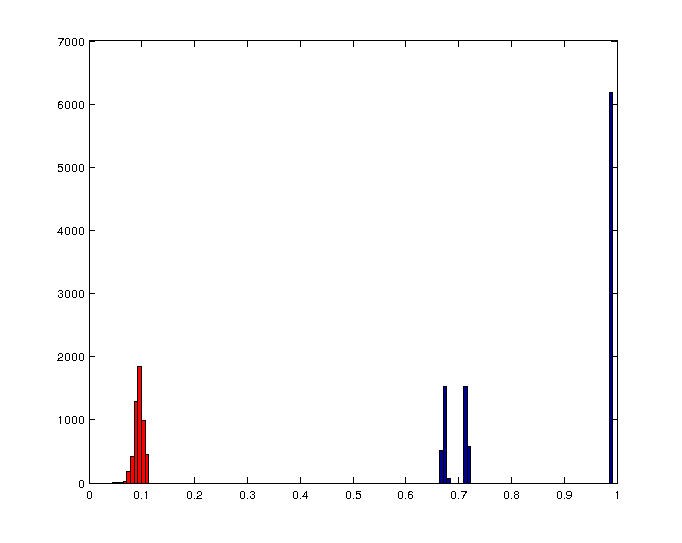
\includegraphics[width=1\textwidth]{ffmpeg-hist}
  \caption{The distribution of the number of differences between original videos (in red) and between original videos and videos processed with ffmpeg (in blue).}\label{fig:ffmpeg-hist}
\end{figure}

The results show that when a video is processed by \emph{Ffmpeg} copying the video stream without re-encoding is enough to greatly alter the file container structure.


\subsection{Exiftool}

\emph{Exiftool} is a command line application for reading, writing and editing metadata information in a variety of media files. With this tool, we have change the creation time information our dataset videos, using the following command:

\begin{lstlisting}
exiftool "-AllDates=1986:11:05 12:00:00" "input.mp4"
\end{lstlisting}

Since we are modifying attributes of the file container that are specific to each unique video, we did not expected this test to perform well. The results are in agreement with this assumption. The changes that \emph{Exiftool} does on a file container are minimal; it just adds a new box at the end of the file, leaving the rest of the structure untouched. As we can see from Fig. \ref{fig:exifaal-hist}, it is not possible to find a threshold that correctly separates the two classes of the binary problem.

\begin{figure}
  \centering
  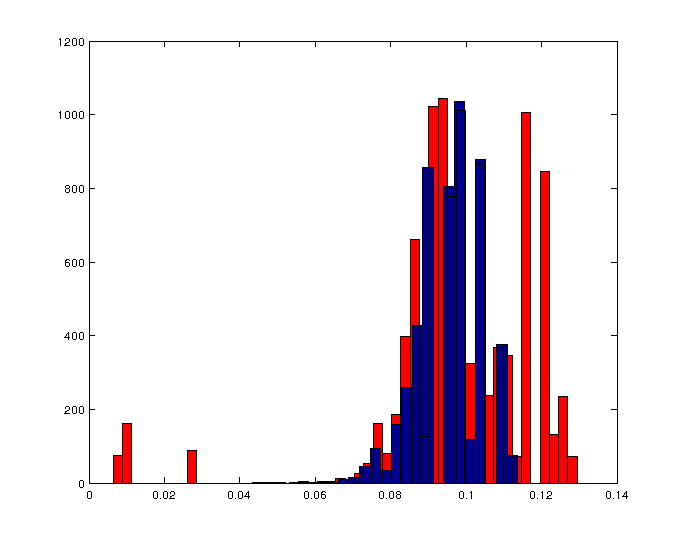
\includegraphics[width=1\textwidth]{exifall-hist}
  \caption{The distribution of the number of differences between original videos (in red) and between original videos and videos processed with exiftool (in blue).}\label{fig:exifaal-hist}
\end{figure}

\begin{figure}
  \centering
  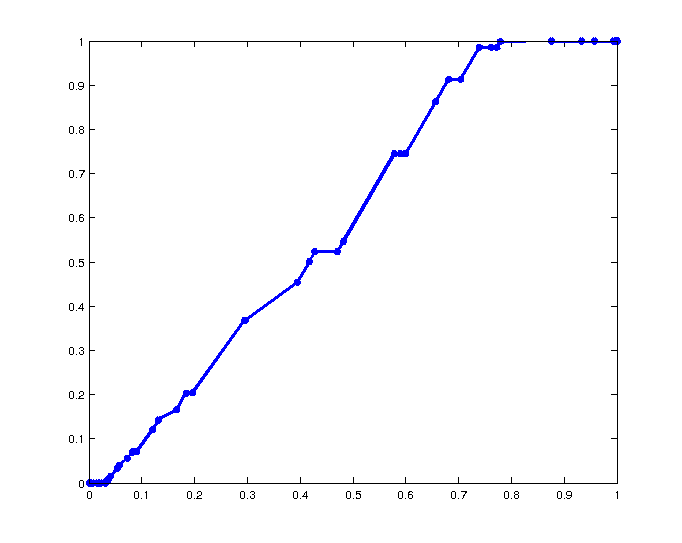
\includegraphics[width=1\textwidth]{exifall-plot}
  \caption{The ROC curve for the experiment with Exiftool shows how the TPR and FPR varies when changing the threshold value.}\label{fig:brand-roc}
\end{figure}

This fact happens because, when we consider all devices, the differences between original videos of the same class for the \emph{Android} devices and for the \emph{iOS} devices have different average values. The additional box that \emph{Exiftool} inserts to the file container for each processed videos adds a constant number of differences for every comparison. This causes the curve associated to the differences between original and processed videos of \emph{Android} devices to overlap the curve associated to the differences between original videos for \emph{iOS} devices.

However, we noticed that the differences between original videos of the same devices regards attributes that are unique to each video, such as \emph{creationTime}, \emph{modificationTime}, \emph{size}, etc. We decided to solve this issue by dynamically build a set composed by attributes whose values are unique to each video for every devices. During the comparison, we will ignore the differences caused by such attributes because their values are not specific to a certain device but to each video.

Without considering such attributes, we are able to separate the two classes with a max accuracy of 1 using a threshold of 0.001.

\section{Source Identification based on File Container}

This section will described the experiments ran to assess the accuracy of our approach with regard to the Source Identification. For each video of the test set we compute the likelihood ratio with respect to every class in the training set. 

When computing the likelihood, the attributes that pertain to the videos and not to the class, as explained previously, will be ignored.

After all the computation have finished, we will obtain a series of likelihood ratios. To each likelihood ratio we need to associate a label accordingly to the class of the test video and the class for which the likelihood have been computed. A label will be 1 the class is the exact brand and model of a test video or is the brand of a test video; it will be 0 otherwise.

Then, using the ROC curve, we determine the threshold value for the likelihood that maximizes the accuracy.

We consider separately the classes that refer to brands and the classes that refer to brands and models, taking into account both manual and automatic mode.

\subsubsection*{Brands}

For manual mode, we obtain a maximum accuracy of 0.9808 with a range of likelihood values between -28 and 32, determine using the results from the ROC curve shown in Fig. (ref).

\begin{figure}
  \centering
  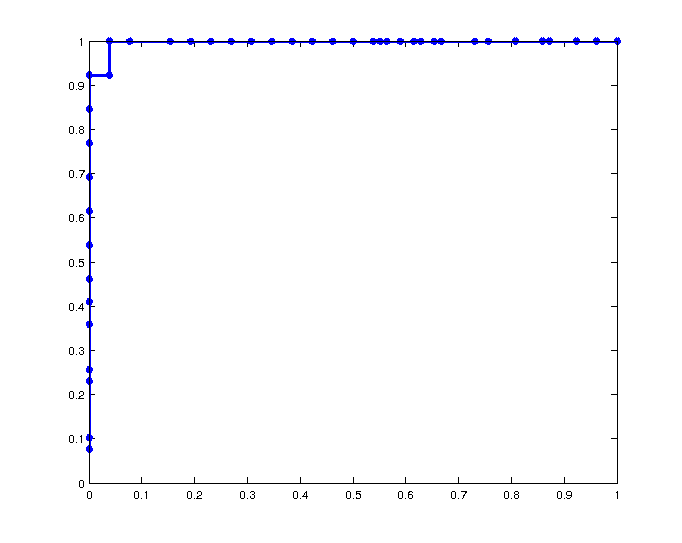
\includegraphics[width=1\textwidth]{brandig-plot}
  \caption{The ROC curve for the experiment with Brands classes shows how the TPR and FPR varies when changing the threshold value.}\label{fig:brand-roc}
\end{figure}

We also determine how precise is the automatic mode by checking the class associated with the higher likelihood ratio. 92\% of the time our method correctly classifies our test videos. For automatic mode, the results can also be visualized in Fig. (ref) where it is shown the confusion matrix. With the confusion matrix we are able to the in which direction the misclassification happened. We can see that the only errors happened because some samsung device are classified as huawei devices. 

\subsubsection*{Brands and Models}

In this case we consider class for which both brand and model are specified. 

For the manual mode, by computing the ROC curve (Fig. \ref{fig:model-roc}, we obtain a maximum accuracy of 0.9754 for a range of likelihood values between 7 and 9.

\begin{figure}
  \centering
  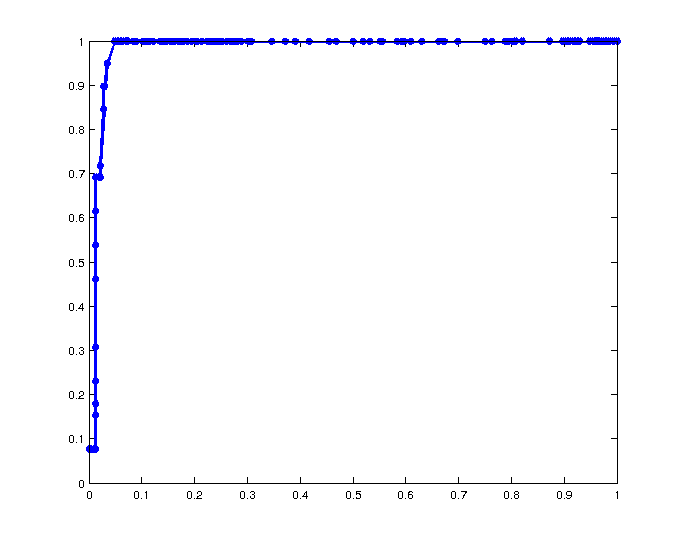
\includegraphics[width=1\textwidth]{modelig-plot}
  \caption{The ROC curve for the experiment with Models classes shows how the TPR and FPR varies when changing the threshold value.}\label{fig:model-roc}
\end{figure}

For the automatic mode, we also determine the precision of our system by computing how many times the correct class is in the top 1 results, in the top 3 results and in the top 5 results. As shown in the table, the correct class is always at least in the top 3 or top 5 and in 84\% of the cases is in the first result.

\section{Application on Social Network}

We have also applied our method to videos that comes from a Social Network, specifically from \emph{Youtube}. The videos of our dataset have been uploaded and then download from \emph{Youtube}.

The experiments have been carried out similarly to the ones for the Integrity Verification. However, we want to determine if videos from \emph{Youtube} are sufficiently similar to be able to distinguish a video that come directly from a source device from a video of that source device that have been subsequently uploaded and downloaded from \emph{Youtube}.

\begin{figure}
  \centering
  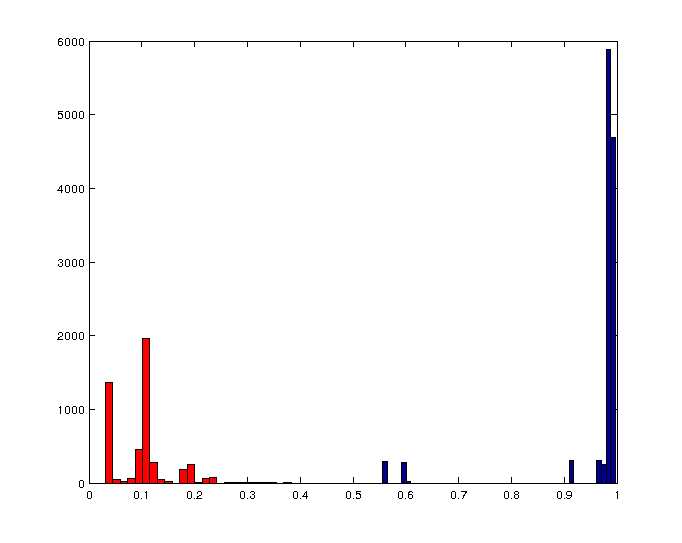
\includegraphics[width=1\textwidth]{youtube-hist}
  \caption{The distribution of the number of differences between \emph{Youtube} videos (in red) and between \emph{Youtube} videos and original videos (in blue).}\label{fig:youtube-hist}
\end{figure}

As can be seen from Fig. \ref{fig:youtube-hist}, the values representing the number of differences between \emph{Youtube} videos and the ones representing the number of differences between original and \emph{Youtube} videos are greatly separated. We obtain a max accuracy of 1 with a range of threshold values between 0.39 and 0.55.
\chapter*{Conclusions}
\addcontentsline{toc}{chapter}{Conclusions}
\chaptermark{Conclusions}

In this thesis, we have proposed an approach for forensic analysis of video file containers. Our method exploits the differences in the file containers structure and content from different manufacturers. In particular, we have dealt with Source Identification and Integrity Verification focused on videos taken from smartphones and tablets.

To implement our method we have developed two Java programs that can be used command line tool, \emph{Video Format Tool} that is used to extract and manipulate the file containers, the \emph{File Origin Analysis} that computes the likelihood that a query video belongs to a certain class of devices. Also, a web application was realized to allow users to easily upload query videos to test.

The experiments show good results for both the Source Identification and the Integrity Verification.

For the Integrity Verification, we have showed that using software editing tools on a video leaves traces on the file container by either adding new boxes or by changing the structure. Our system is always able to detect the changing in the file container structure of a minimally processed video when compared to a reference video. 

For Source Identification, we were able to correctly classify our test videos based on their file containers in most cases. The misclassifications are due to different manufacturers using a very similar structure for the file containers. Also, how the reference population is built during the training phase might cause some errors. It is possible that having a more varied dataset in terms of devices with a greater number of videos per device will lead to a more accurate classification.

Although we get good results, this thesis should be considered preliminary work whose main intent is to show that using file containers for forensic analysis of digital video is an interesting approach. In fact, there are many aspect that could be improved and investigated more:

\begin{itemize}

\item Some boxes are only present in the file containers when a particular condition happens during the acquisition of the video. Such is the case of the box \emph{xyz} that contains information about the GPS coordinates and that is located inside the User Data Box (\emph{udta}). This box is only present if, during the acquisition of the video, localization was active on the device. Given a file container, the presence or the absence of such box does not give us any information about the source device. However, adding the box \emph{xyz} means adding the box \emph{udta}, located inside the Movie Box (\emph{moov}). Since we are using an indexing to determine the position of a box, this addition causes all the box indexs to shift. So two videos taken from the same device, one using GPS location and the other not, have very different file container representation for our system that sees them as coming from distinct sources. Right now, this issue is resolve with a workaround that will ignore the box \emph{xyz}. However, there is the need to implement a more elegant and extensible solution that can deal with other unknown boxes that behave the same.

\item One aspect that could be improved is how the attributes values are compared. Right now some attributes that are related only to the specific video, such as \emph{creationTime} or \emph{duration}, are ignored. An improved solution might be implementing a comparator function that specializes in a different way accordingly with the kind of attribute under consideration. For example, comparing values for the attribute \emph{flag} is different from comparing value of the attribute \emph{creationTime}. For the first, it is sufficient to directly confront the values and check if they differ or not; for the latter, it might be a better idea to check whether the dates are in the same format. In this way, we remove the need to ignore certain attributes and we could also improve the performance of our approach because we would be able to access more information.

\item The dataset we used for experiments is limited in terms of number of videos but more specifically in terms of types of devices. It would be interesting to try our method when more devices from different brands and models are available. Moreover, for the videos in our dataset only the generic operating system is known. We do not possess information about the version of the operating systems for each video. Changing the version of an operating system could also mean changes in the file container. We could harness this information to allow us to be even more specific in identifying the source device for a query video.

\item The problem of how to create the reference population is still open. We notice that based on how the reference population is built, the discriminant powers of the attributes change and so changes the computed likelihood given a query video.
It might be possible to find a more systematic way to determine the reference population or even to developed a method that allow us to use the entire population as a reference without losing in performance.

\end{itemize}


}

%%%  BACK MATTER  %%%  (bibliografia)
\backmatter

{
\bibliographystyle{style/ieee}
\bibliography{main/bibliography}
}

\chapter*{Credit}
\addcontentsline{toc}{chapter}{Credit}
\chaptermark{Credit}

\end{document}

%pagina bianca (da usare, nei punti giusti, x avere una pag bianca invece che vuota con intestazione)
%\newpage{ \thispagestyle{empty}\null\vfil}